
\documentclass{exam}

\usepackage{units} 
\usepackage{graphicx}
\usepackage[fleqn]{amsmath}
\usepackage{cancel}
\usepackage{float}
\usepackage{mdwlist}
\usepackage{booktabs}
\usepackage{cancel}
\usepackage{polynom}
\usepackage{caption}
\usepackage{fullpage}
\usepackage{xfrac}
\usepackage{enumerate}

\newcommand{\degree}{\ensuremath{^\circ}} 
\everymath{\displaystyle}

% \begin{figure}[H]
%   \centering
%   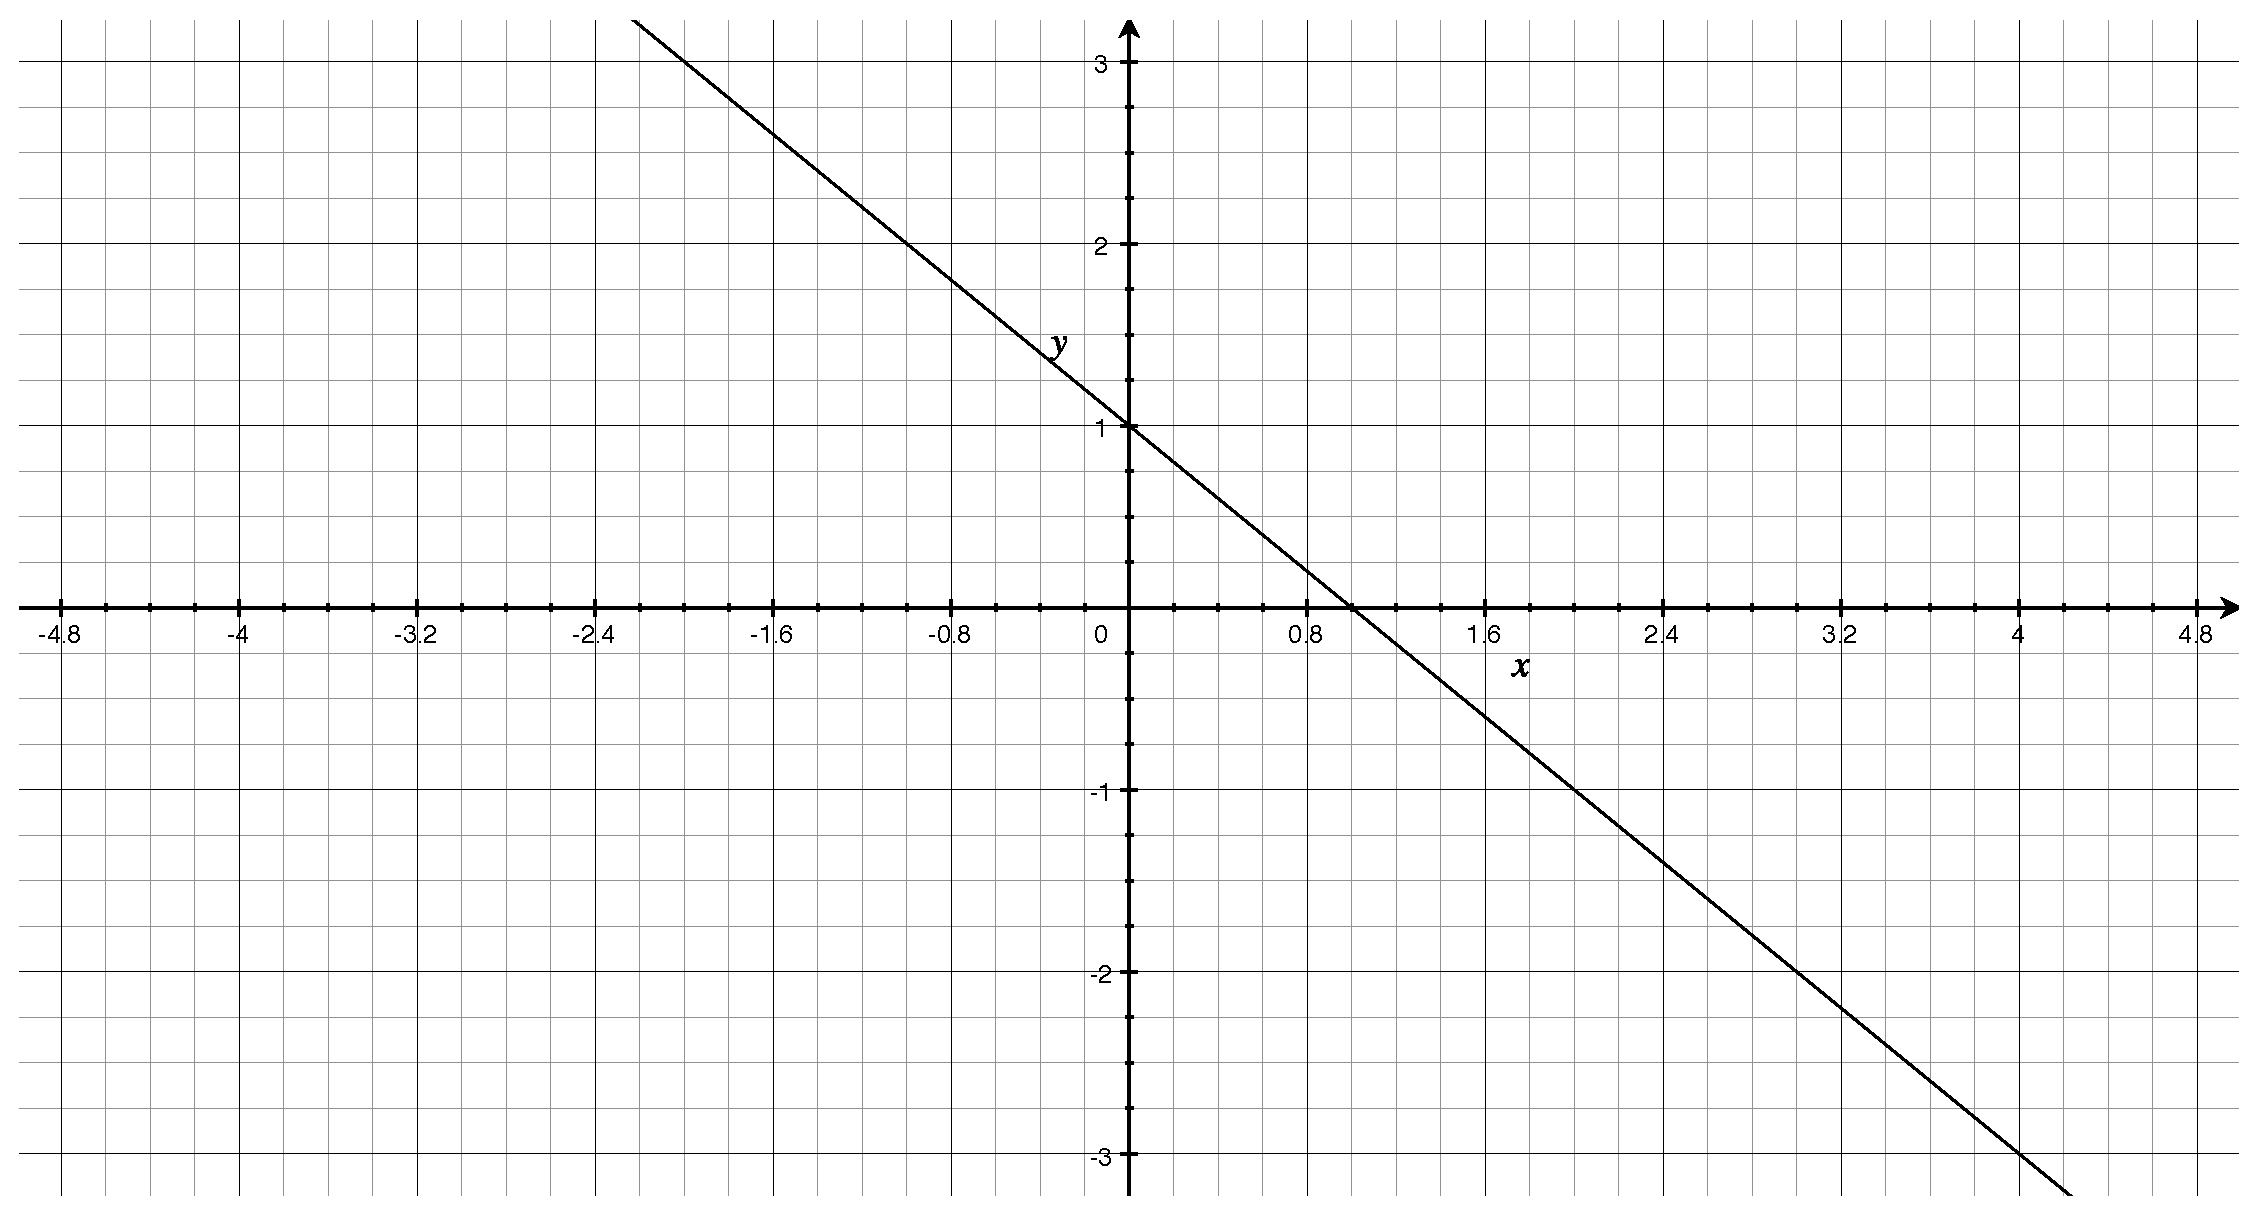
\includegraphics[scale=0.9]{problem7.eps}
%   \caption*{Problem 7}
% \end{figure}

% \begin{tabular}{cc}
%   \toprule
%   period & amplitude \\
%   \midrule
%   value one & value two
%   \bottomrule
% \end{tabular}

% \printanswers

\ifprintanswers 
  \usepackage{2in1, lscape} 
\fi

\date{June 5, 2013}
\author{}
\title{Math 141 \\ Homework 13}

\begin{document}

  \maketitle

  \section{Homework}

  Section 4.2: 

  \section{Extra Credit}
  Section 4.2, TO DO

  \ifprintanswers
    \begin{description}
      \item[49] TO DO
    \end{description}

  \section{Review}

  \begin{enumerate}
    \item Simplify: $\frac{\sqrt{-4}\sqrt{-27}\sqrt{-16}}{\sqrt{-3}}$
      \begin{solution}
        \begin{align*}
          \frac{\sqrt{-4}\sqrt{-27}\sqrt{-16}}{\sqrt{-3}} &= \frac{2i \cdot 3i \sqrt{3} \cdot 4i}{i \sqrt{3}} \\
          &= \frac{24i^3 \sqrt{3}}{i \sqrt{3}} \\
          &= 24 i^2 \\
          &= -24 \\
        \end{align*}
      \end{solution}

  \end{enumerate}
    \section{Section 4.2}

    \begin{description}

      \item[3] 
        \begin{itemize}[a]
          \item $5^2 = 25$
          \item $5^0 = 1$
        \end{itemize}

    \item[4] 
      \begin{itemize}[a]
        \item $10^{-1} = 0.1$
        \item $8^3 = 512$

      \end{itemize}

    \item[5] 
      \begin{itemize}[a]
        \item $8^{1/3} = 2$
        \item $2^{-3} = \frac{1}{8}$
      \end{itemize}

    \item[6] 
      \begin{itemize}[a]
        \item $4^5 = 81$
        \item $8^{2/3} = 4$
      \end{itemize}

    \item[7] 
      \begin{itemize}[a]
        \item $e^x = 5$
        \item $e^5 = y$
      \end{itemize}

    \item[8] 
      \begin{itemize}[a]
        \item $e^2 = x + 1$
        \item $e^4 = x - 1$
      \end{itemize}

    \item[9] 
      \begin{itemize}[a]
        \item $\log_5 125 = 3$
        \item $\log_{10} 0.0001 = -4$
      \end{itemize}

    \item[10] 
      \begin{itemize}[a]
        \item $\log_{10} 1,000 = 3$
        \item $\log_{81} 9 = \frac{1}{2}$
      \end{itemize}

    \end{description}


  \else
    \vspace{6 cm}
    \begin{quote}
      \begin{em}
        TO DO
      \end{em}
    \end{quote}

    \hspace{1 cm} --Henry David Thoreau
  \fi

\end{document}

